% <!-- This makes it look pretty in a browser --><pre>
\documentclass[a4paper,english]{cv}
\usepackage[latin1]{inputenc}
\usepackage{a4wide}
\pagestyle{empty}
\usepackage{graphicx}
\usepackage{longtable}
\makeatletter
\newcommand{\HS}{\hspace{0.5cm}}
\date{}
\newcommand{\B}[1]{%
\makebox[1cm][l]{\small{#1:}}}
\newcommand{\VT}{\vspace{2mm}}
\renewcommand{\topicmargin}{7em}
\usepackage{babel}
\makeatother
\begin{document}
\title{Curriculum Vitae}
\maketitle
\thispagestyle{empty}\centerline{\fbox{\begin{minipage}[c]{0.50\columnwidth}%
\begin{center}\hfill{}\hfill{}\begin{tabular}{p{2.1cm}p{4cm}}
Name:&
Martin Strauss\\
Address:&
\parbox[t]{4cm}{Karcherstra�e 16
\\
66111 Saarbr�cken
\\
GERMANY\VT{}}\\
Telephone:&
\parbox[t]{4cm}{Home: +49 681 5006 376
\\
Mobile: +49 163 1462 550\VT{}}\\
E-mail:& martin@ockle.org\\
Birth:& 19th July, 1983; K�ln, Germany\\
Citizenship:& Australian (naturalised 26th January 1988)\\
\end{tabular}\hfill{}\end{center}\end{minipage}%
\begin{minipage}[c]{0.50\columnwidth}%
~\hfill{}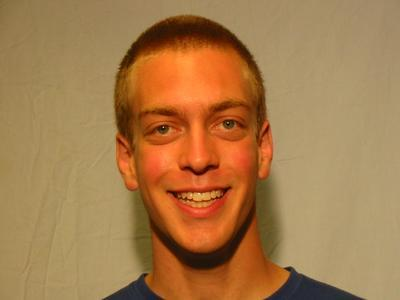
\includegraphics[%
  width=0.50\columnwidth,
  keepaspectratio]{Strauss_Martin.jpg}\hfill{}~\end{minipage}%
}}
\section{Professional Interests}

Software quality and usability: in particular, post-desktop interaction styles such as haptics, non-speech audio, and embodied agents.\section{Education}

\begin{topic}
\item [2006 -- 2007]\textbf{Master of Science} The University of Saarland and Max Planck Institute for Computer Science

Awarded International Max Planck Research School Scholarship.
Masters thesis: ``Realtime generation of multimodal affective sports commentary for embodied agents''.
Graduated with honours.

\item [2004 -- 2005]\textbf{Taste of Research Summer Scholarship} The University of New South Wales and National ICT Australia

I investigated the technologies and applications of the field of affective computing (the use of emotions in AI and interface design).  I produced a preliminary ontology of affective computing concepts, for use in a hypothetical agent or affective application.  The results of my work were presented at a poster session at UNSW, and in a report titled ``The Logics of Emotion: a survey of the field of Affective Computing''(see Publications below, \emph{{[}2{]}})

\item [2001 -- 2005]\textbf{Bachelor of Engineering (Software), Diploma of
    Music (Practical)} The University of Melbourne

Graduated 2005 with first class Honours.

\begin{itemize}
\item Ormond Scholar, Ormond College, 2001, 2003 -- 2005
\item Choral Scholar, Ormond College, 2001 -- 2005
\item MacFarland Scholar, Ormond College, 2005
\item McCaughey Scholar, Ormond College, 2004
\item Music Scholar, Ormond College, 2002
\item Centenary Scholar, Ormond College, 2001
\item School Music captain, Geelong Grammar School, 2000
\end{itemize}
\item [1999 -- 2000]\textbf{Melbourne University Program for High Achieving Students} The University of Melbourne

First year Music Performance, Piano, 1999 (first class Honours); and First Year Mathematics, 2000 (second class Honours, division A)

\item [1999 -- 2000]\textbf{International Baccalaureate} Geelong Grammar School

Score of 44 out of possible 45 with perfect subject scores in 5 of 6 subjects, as well as perfect scores for the Extended Essay and Theory of Knowledge.

Title of Extended Essay: ``An investigation into matrix encryption for the purpose of enciphering text messages''(see Publications below, \emph{{[}1{]}})

\item [1994 -- 2000]\textbf{Geelong Grammar School} \begin{itemize}
\item Academic Scholarship, 1994 -- 2000
\item Music Scholarship, 1995 -- 2000
\item Senior Chorister, the Choir of Ormond College, 2003 -- 2005
\end{itemize}
\item [1989 -- 1993]\textbf{The Geelong College} \end{topic}

\section{Other Training}

\begin{topic}
\item [December 2004] The Australian Logic Summer School

As part of my National ICT Australia Summer Scholarship, I attended the Australian Logic Summer School at the Australian National University's Research School of Information Sciences and Engineering.  There, I participated in lectures, workshops and seminars on the mathematical and philosophical foundations of logic, and a wide variety of applications of logic in computing, including theorem proving, constraint programming, artificial intelligence and knowledge representation and reasoning.

\item [February 2002] SecureCON

I attended the inaugural University of Melbourne Local IT Experts Security Convention, and participated in seminars and workshops on topics such as securing webservers, using intrusion detection systems, using network traffic monitors, writing a information security policy and managing a security compromise.

\item [April 2000] Australian Business Week

I was one of 66 Victorian students awarded a scholarship to participate in the Australian Business Week. This is a one-week intensive residential program aimed at developing the entrepreneurial and small business culture of young Australians. During this program, I also participated in a Team Skills Development workshop.

\end{topic}
\section{Employment}

\begin{topic}
\item [2007 --] \textbf{Software Engineer, Google Inc.}  Freigutstrasse 12, CH-8002 Z�rich, Switzerland

I work as a software engineer in the iGoogle group at Google.  We aim to improve the user experience at the Google home page, and investigate and develop new ways of interacting with Google products.

\item [2006 -- 2007] \textbf{Research Assistant, Deutsche Forschungszentrum f�r K�nstliche Intelligenz}  Stuhlsatzenhausweg 3 (Geb�ude D3 2)
D-66123 Saarbr�cken, Germany

I worked as a research assistant (wissenschaftliche Hilfskraft) at the German research center for AI (DFKI) in the VirtualHuman group, developing software tools for creating, deploying and evaluating the embodied agents ("Virtual Human") developed by the group.

\item [2006] \textbf{Software Engineer, Defence Science and Technology Organisation}  506 Lorimer St, Fishermans Bend VIC 3207, Australia

From January until March I worked as a graduate software engineer in the Air Operations Simulations Center in the Defence Science and Technology Organisation.  The Air Operations Simulations Center operates a facility in which cutting-edge technology is used to produce a realistic flying environment for human-in-the-loop simulation experiments.  The facility conducts research into aerospace operations requirements and equipment suitability for Australian Defence aerospace operations.

\item [2005] \textbf{Tutor, Ormond College}  College Crescent, Parkville, VIC 3052, Australia

During the second semester of 2005, I tutored a group of first year students at Ormond College who were taking the subject `Electrical Circuits'.  In their end-of-term feedback, the students wrote that I `helped [them] to raise questions, express uncertainties and participate fully', and that the tutorials were `stimulating and thought provoking'.

\item [2004 -- 2005] \textbf{Software Engineering Project and Advanced Software Engineering Project}  

As part of my Software Engineering degree at the University of Melbourne, I participated in two industrial projects.  In the first, I was in a team of 5 software engineers who developed a software package for researchers in the Optics group in the School of Physics at Melbourne University.  For the second, I was in a team of 15 software engineers who developed a software package for researchers in the Department of Information Systems at Melbourne University.  In each project, We conducted all of the activities of the software and project lifecycle, including planning and managing the software process, requirements elicitation, documentation, requirements analysis, specification, design, implementation and testing.  As part of both projects, we were required to communicate effectively both with each other and with the client, and undertake a variety of leadership positions during the course of the project.  As technical manager and Executive Officer of the first team, my tasks included training the other team members in the tools and software used during the project, supervising team ``work sessions'', and setting and monitoring weekly team goals and objectives; as quality assurance manager and build manager in the second team, my tasks included setting quality objectives for our product, developing, documenting, monitoring and improving quality  processes for our team, and overseeing and managing the tasks and schedule for the final build of our software system.

\item [2001 -- 2005] \textbf{IT Administrator, Ormond College}  College Crescent, Parkville, VIC 3052, Australia

I worked in the IT administration department at Ormond College, first as Assistant IT Administrator in 2001, then as IT Administrator from 2002 onwards. As well as administering a network consisting of several Linux servers, a computer room of 15 Windows NT/2000 workstations, 15 employee Windows workstations and a variable number of student workstations (Windows, Mac and Linux), I participated in the planning and implementation of an LDAP-based authentication and mail routing system, and later in the planning and implementation of a full network hardware upgrade from 10Mbps unswitched to 1Gbps backbone and 100Mbps to the desktop, fully switched, including the extension of the LAN to include a number of terrace houses in the surrounding suburbs owned by Ormond College.

\item [Summer 1999, 2000] \textbf{Laboratory Assistant, Rohm and Haas Australia Pty. Ltd.}  Hays Road, Point Henry, Geelong, VIC 3220, Australia

During the 1999/2000 and 2000/2001 summer holidays, I worked for Rohm and Haas Australia Pty Ltd in their Geelong Technical Centre. I assisted industrial chemists with research and technical service projects, working at the cutting edge of paint technology.

\end{topic}

\section{Other positions held}

\begin{topic}
\item [2003] \textbf{Head of Pleasant Sunday/Wednesday Evening Subcommittee of the Ormond College Students' Club}

As head of the PS/WE subcommittee, I was responsible for organising a series of relaxed social events throughout the academic year for the members of the Ormond College Students' Club.  I was required to write and work with a budget for these events, and manage a subcommittee of around 20 members to organise venues, food and beverages, and entertainment.

\item [2003 -- 2005] \textbf{Senior Chorister, the Choir of Ormond College}

In addition to singing with the Choir of Ormond College, as Senior Chorister I
had the responsibility of assisting the Director of the Choir in a variety of ways, including managing the Friends of the Ormond Choir and writing an annual newsletter; organising choir events, a choir contact list, etc; assisting the Director in organising concerts and a biennial overseas concert tour; organising the Choir's rehearsals and occasionally leading the Choir in rehearsals; and conducting the Choir in the Director's absence.

\item [2000] \textbf{School Music captain, Geelong Grammar School}

As co-School Music Captain of GGS, I was responsible for assisting the Director of Music in the running of the Music School and musical events, including leadership on the 2000 Choir concert tour of Europe; leadership and organisation of musical groups; MC-ing at various events and functions; and organisation and occasional leadership of rehearsals.

\end{topic}

\section{Publications}

\begin{topic}
\item [{[}1{]}]Martin Strauss, \emph{An investigation into matrix encryption for the purpose of enciphering text messages}. International Baccalaureate Extended Essay, Geelong Grammar School, November 2000.

\item [{[}2{]}]Martin Strauss, \emph{The Logics of Emotion: a survey of the field of Affective Computing}. University of NSW Taste Of Research Summer Scholarship report, February 2005.

\end{topic}

\section{Skills}
\subsection{Computer Skills}

\begin{topic}
\item [ OS]  Expert user of Unix (especially Linux and SunOS) and Mac OS X, advanced user of Windows.

\item [ Languages]  Extensive experience with C, Java, C++, Prolog, Javascript, PHP, Python and Perl, as well as BASH shell scripting. Also experience with languages such as Haskell, Lex/Yacc, BASIC, RSI IDL and Assembler (primarily x86) as well as some exposure to Pascal, Scheme, Lisp, etc.

\item [ Software Engineering]  Extensive experience with UML and Object-Oriented design, agile development methods, and also with functional and logic programming.  Also experience with Microsoft Visual Studio, Rational Rose, Eclipse, NetBeans.

\item [ Administration]  Extensive experience administering Linux servers (primarily Debian GNU/Linux and Gentoo, but also Red Hat, Mandrake and Slackware), and some experience administering Windows NT4, 2000 and XP workstations and Windows NT4, 2000 and 2003 servers. Experience with directory services (LDAP), SQL databases (MySQL and PostgreSQL), firewalls and routing (netfilter/iptables and ipfilter), Internet proxy services (squid, dante-socks), mail services (sendmail, exim, postfix), etc.

\item [ Tools]  Experience using and programming MATLAB and RSI IDL, and toolboxes such as Simulink.

\end{topic}
\subsection{Language Skils}

\begin{topic}
\item [ English]  native language

\item [ German]  native language

\item [ Japanese]  some knowledge

\end{topic}
\section{Professional Associations}

\begin{topic}
\item [1995 -- 2001] \textbf{Member of the CSIRO Double Helix Science Club} 

\item [2001 -- 2005] \textbf{Member of Melbourne University Young Engineers} 

\item [2001 --] \textbf{Student Member of the Association of Professional Engineers, Scientists and Managers} 

\item [2001 --] \textbf{Student Member of the Institute of Engineers, Australia} 

\end{topic}
\section{Interests}

\subsection{Music}

\begin{itemize}
\item I began learning piano when I was four years old, and flute when I was 8.  I achieved Licentiate Diploma level in piano and Associate  Diploma level in flute by the time I was 12 years old.  I've given many public performances both on piano and flute and achieved considerable success in competitions on both instruments.  I have participated in the Piano Masterclass Series (on full scholarship) at the Australian National Academy of Music since 1999.
\item I was an active participant in music groups at school: I was School Music Captain in 2000.  I was a member of the Geelong Grammar School Concert Band, the Geelong Grammar School Orchestra and the Concert Choir of Geelong Grammar School.  I participated in the Concert Choir tour through Europe in June/July 2000, culminating in the 29th International Youth and Music Festival in Vienna, where we were runner-up in the mixed Choir section.
\item From 2001 to 2005 I sang in (and from 2003 to 2005 was Senior Chorister of) the Choir of Ormond College at The University of Melbourne: The Choir sings an annual concert series in Melbourne and country Victoria.  I have toured Europe with the Choir of Ormond College three times, in 2001, 2003 and 2005.  I have participated in the recording of three CDs with the Choir of Ormond College.
\end{itemize}

\subsection{Sport}

\begin{itemize}
\item I am a keen touring cyclist and participated in four of Bicycle Victoria's Great Victorian Bike Rides (1995,1996, 1997 and 2000) over 9 days, as part of a Geelong Grammar School Team.  In 1997 I successfully completed the Around the Bay in a Day ride (210 km in one day), in support of the Smith Family's fundraising for underprivileged families.
\item As a member of the University of Melbourne Ultimate Frisbee Club, I have regularly played in the Victorian Flying Disc Association's Competitive League on a University of Melbourne team.  I represented the University of Melbourne in the Australian University Games 2002 in Ultimate Frisbee.
\end{itemize}

\subsection{Community}

\begin{itemize}
\item I have performed piano recitals on a voluntary basis, on several occasions for St Laurence Park Aged Care Services, Lara.
\item I have carried out volunteer work for the Sanctuary, Geelong, helping
with fundraising events.
\item During 1999, together with a group of students I began working with CREATE unemployment services in Corio to establish a free Internet cafe. We raised funds to buy several computers and an Internet connection, and were able to set up a pleasant facility where young unemployed people could meet and easily access the Internet.
\item In 1997 I carried out volunteer work for the Department of Forestry and Lands on huts and campsites in Victoria's high country.
\end{itemize}

\section{University Marks}

\begin{longtable}{|l|l|r|l|}
\hline code& subject title& mark& grade\\
\hline
\hline \endhead
740136&  Music Performance 1& 89&  H1\\ 
\hline 620120&  MUPHAS Mathematics& 76&  H2A\\ 
\hline 431102&  Digital Electronics and Microprocessors& 75&  H2A\\ 
\hline 433141&  Computing Fundamentals A& 89&  H1\\ 
\hline 436105&  Engineering Communications& 88&  H1\\ 
\hline 620143&  Applied Mathematics& 82&  H1\\ 
\hline 431103&  Electrical Circuits& 68&  H3\\ 
\hline 431201&  Engineering Analysis A& 74&  H2B\\ 
\hline 433142&  Computing Fundamentals B& 89&  H1\\ 
\hline 436101&  Engineering Mechanics and Materials& 72&  H2B\\ 
\hline 740104&  Ensemble 1-1& 87&  H1\\ 
\hline 740103&  Ensemble 1-2& 95&  H1\\ 
\hline 740146&  Practical Study 1D& 90&  H1\\ 
\hline 431202&  Engineering Analysis B& 62&  P\\ 
\hline 431204&  Digital Systems 2: System Design& 69&  H3\\ 
\hline 436202&  Mechanics 1& 63&  P\\ 
\hline 436280&  Mechatronics Design and Laboratory& 52&  P\\ 
\hline 431221&  Fundamentals of Signals and Systems& 71&  H2B\\ 
\hline 433252&  Software Engineering Principles and Tools& 90&  H1\\ 
\hline 436201&  Thermofluids 1& 74&  H2B\\ 
\hline 436281&  Mechatronics Design and Laboratory 2& 68&  H3\\ 
\hline 740204&  Ensemble 2-1& 92&  H1\\ 
\hline 740203&  Ensemble 2-2& 90&  H1\\ 
\hline 740246&  Practical Study 2D& 90&  H1\\ 
\hline 433253&  Algorithms and Data Structures& 69&  H3\\ 
\hline 433254&  Software Design& 89&  H1\\ 
\hline 433255&  Logic and Computation& 76&  H2A\\ 
\hline 433353&  Networks and Communications& 76&  H2A\\ 
\hline 433361&  Programming Language Implementation& 86&  H1\\ 
\hline 433371&  Interactive System Design& 87&  H1\\ 
\hline 640142&  Physics B& 81&  H1\\ 
\hline 740308&  Ensemble 3-1& 90&  H1\\ 
\hline 740344&  Ensemble 3-2& 90&  H1\\ 
\hline 740346&  Practical Study 3D& 82&  H1\\ 
\hline 433330&  Theory of Computation& 80&  H1\\ 
\hline 433341&  Software Engineering Process and Practice& 75&  H2A\\ 
\hline 433343&  Professional Issues in Computing& 82&  H1\\ 
\hline 433303&  Artificial Intelligence& 83&  H1\\ 
\hline 433342&  Software Engineering Methods& 77&  H2A\\ 
\hline 740315&  Romantic Piano Music& 80&  H1\\ 
\hline 433340&  Software Engineering Project& 88&  H1\\ 
\hline 433441&  System Modelling and Analysis & 82&  H1\\ 
\hline 433443&  Software Project Management& 82&  H1\\ 
\hline 433448&  Applied Cryptography and Coding& 85&  H1\\ 
\hline 433440&  Advanced Software Engineering Project A& 78&  H2A\\ 
\hline 433471&  Logic Programming& 73&  H2B\\ 
\hline 740301&  Music and Film& 90&  H1\\ 
\hline 433444&  Advanced Software Engineering Project B& 78&  H2A\\ 
\hline 650& Automated Debugging& -& 1.0\\ 
\hline 559& Security& -& 2.7\\ 
\hline 5001& Intelligent Tutoring Systems& -& 1.0\\ 
\hline 5002& Intelligent Environments& -& 1.0\\ 
\hline 5003& Empirical Software Engineering& -& 1.7\\ 
\hline 
\end{longtable}

\section{Awards}

\subsection{Geelong Grammar School Awards}

\begin{itemize}
\item Triple Distinction Prize (1996)
\item Distinction Prize (1995, 1997)
\item Double Distinction Prize (1998)
\item General Academic Excellence Award
\item School colours for Public Speaking
\item School colours for Music
\item School colours for Debating
\item School colours for Academic Work
\item Distinctions in English (1995, 1996, 1997, 1998), Mathematics (1995,
1996, 1997, 1998, 1999), Science (1995, 1996), Japanese (1995, 1996,
1997, 1998), Music (1995, 1996, 1997), Religious Education (1996),
Geography (1996), History (1997, 1998), Physics (1998, 2000), Chemistry
(1998), Music Performance (1998), Economics (1999).
\item Mackinnon Prize for Mathematics
\item Charles Murray Maxwell Prize for Chemistry
\item ANZ Bank Prize for Economics
\item I M Cook Prize for Music
\item Academic Scholarship, 1994 -- 2000
\item Music Scholarship, 1995 -- 2000
\end{itemize}

\subsection{The University of Melbourne Awards}

\begin{itemize}
\item Centenary Scholar, Ormond College, 2001
\item Music Scholar, Ormond College, 2002
\item McCaughey Scholar, Ormond College, 2004
\item MacFarland Scholar, Ormond College, 2005
\item Ormond Scholar, Ormond College, 2001, 2003 -- 2005
\item Choral Scholar, Ormond College, 2001 -- 2005
\end{itemize}

\subsection{Other Academic Awards}

\begin{itemize}
\item Winner, Mathematical Association of Victoria Maths Talent Quest (1993)
\item Distinction, NAB Languages Certificate (1996)
\item Member of winning team, Deakin University Mathematics Competition
(1998)
\item Special Achievement Award (highest school score), Australian Mathematics
Competition (Australian Mathematics Trust) (1999)
\item Member of runner-up team (and winners of the Judges' Prize), Melbourne
University Mathematics Society puzzle hunt (2004)
\end{itemize}

\subsection{Miscellaneous Awards}

\begin{itemize}
\item Duke of Edinburgh Award, Bronze Medal (1997)
\end{itemize}

\subsection{Music Awards}

\begin{itemize}
\item AMEB Pianoforte Diploma, Associate in Music, Australia (AMusA), October
1994
\item Chosen from Australia-wide as one of twenty "outstanding
young musicians" for Asia-Australia Culture and Arts Centre
tour of People's Republic of China (1996)
\item AMEB Flute Diploma, Associate in Music, Australia (AMusA), May 1996
\item AMEB Pianoforte Diploma, Licentiate in Music, Australia (LMusA), September
1996
\item Selected to participate in the National Academy of Music Piano Master
Classes, (1999 -- 2004)
\item Finalist, Yamaha Australian Youth Piano Championship (1999)
\item Winner, Lions Club Scholarship, Dandenong Festival of Music and Art
for Youth (2001)
\item Winner, Dorothy Glover Piano Scholarship (2001)
\item Finalist, Lev Vlassenko International Piano Competition (2001)
\item Finalist, Hephzibah Menuhin Memorial Awards (several occasions)
\item Winner, Australian Youth Pianoforte Recital, Dandenong Festival of
Music and Art for Youth (2002)
\item Winner, Gold Medallion for most outstanding Pianist in the festival,
Dandenong Festival of Music and Art for Youth (2001, 2002)
\item Runner-up, Geelong Advertiser Music Scholarship (2002)
\item Winner, Highton Rotary Club annual Star Search (2002)
\end{itemize}

\end{document}
%</pre><!-- This makes it look pretty in a browser -->
